% assignment_4.tex - Assignment 4 for Machine Learning class (Spring 2015)
% Chanmann Lim - April 2015

\documentclass[a4paper]{article}

\usepackage[margin=1 in]{geometry}
\usepackage{amsmath}
\usepackage{listings}
\usepackage{graphicx}
\usepackage[T1]{fontenc}
\usepackage{float}
\usepackage{multirow}
\usepackage{rotating}

\everymath{\displaystyle}

\begin{document}
\subsection*{2.}

% Iris training dataset consists of 90 samples from homework 3 is used to conduct the Principal component analysis (PCA) using $PCA$ function from Classification toolbox to obtain $W$ transformation matrix.\\
% \paragraph{a.}
% \paragraph{b.} To reduce the dimension of the test samples, we need to  \\
% \paragraph{c.} ~\\
% \paragraph{d.} ~\\
\paragraph{e.} Confusion table: \\

\begin{tabular}{|r| *{3}{c|}}
  \hline
  \multirow{2}{*}{True class} 
        & \multicolumn{3}{ c| }{Classified class} \\ \cline{2-4}
        & Setosa & Versicolor & Virginica\\ \hline
  Setosa    & 20 &  0 &  0\\ \hline
  Versicolor  &  0 & 20 &  0\\ \hline
  Virginica &  0 &  0 & 20\\ \hline
  
\end{tabular}
\paragraph{f.} Scatter plot for the PCA projected Iris data: \\

\begin{figure}[H]
  \centering
    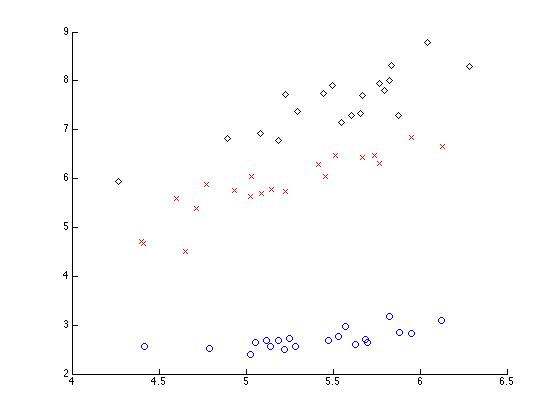
\includegraphics[scale=.47]{images/2_f.png}
  \caption{2D projected test dataset}
\end{figure}
\paragraph{g.} The original 4D Iris test dataset was projected into 2D data samples using PCA before classification task is performed and for the given set of test data we found that there is no classification error using MLE classifier which can be seen from the scatter plot and the confusion table.\\

% -------------------------------- 3 --------------------------------
\subsection*{3.}
\paragraph{c.} The classification task of the Iris data is a 3-class classification problem and for the Multiple discriminant analysis which is a generalization of Fisher's linear discriminant involves (3-1) discriminant functions hence the dimensionality of projection is not possible to get up to 3. \\
\paragraph{e.} Confusion table (MDA): \\

\begin{tabular}{|r| *{3}{c|}}
  \hline
  \multirow{2}{*}{True class} 
        & \multicolumn{3}{ c| }{Classified class} \\ \cline{2-4}
        & Setosa & Versicolor & Virginica\\ \hline
  Setosa    & 20 &  0 &  0\\ \hline
  Versicolor  &  0 & 20 &  0\\ \hline
  Virginica &  0 &  0 & 20\\ \hline
  
\end{tabular}
\paragraph{g.} Scatter plot for the PCA projected Iris data with MDA: \\

\begin{figure}[H]
  \centering
    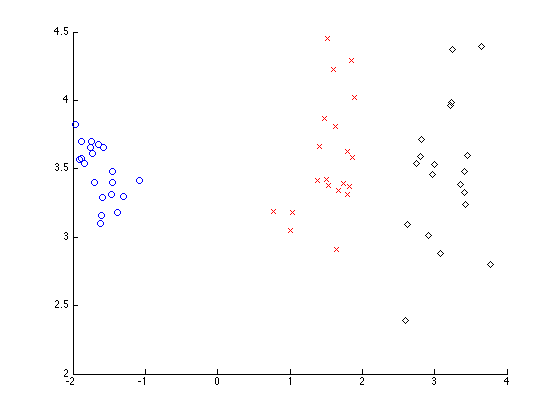
\includegraphics[scale=.47]{images/3_g.png}
  \caption{2D projected test dataset}
\end{figure}
\paragraph{h.} Same as the classification result of the PCA function, projected 2D dataset produced by MDA function also work really well with MLE classifier and we could also get zero classification error for the given dataset.\\

\subsection*{4.}
\paragraph{b.} Display original and approximated images: \\
\begin{figure}[H]
  \centering
    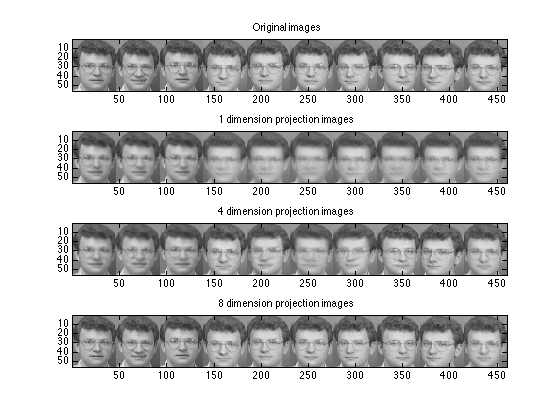
\includegraphics[scale=.67]{images/4_b.png}
  \caption{Original and approximated images}
\end{figure}

\paragraph{c.} Proportion of variances(beta\_k) and approximation error(e\_square). \\

\begin{verbatim}
k:1 => beta_k = 0.40158, e_square = 631257.3661
k:4 => beta_k = 0.78715, e_square = 224526.7043
k:8 => beta_k = 0.98096, e_square = 20080.7289
\end{verbatim}


\subsection*{5.}
\paragraph{c.} Classification error rate summary: \\

\begin{tabular}{|r| *{3}{c|}}
  \hline
  \multirow{2}{*}{\# of nearest neighbors} 
        & \multicolumn{3}{ c| }{\# of features} \\ \cline{2-4}
        & 1 & 4 & 10\\ \hline
  1    & 0.32 &  0 &  0\\ \hline
  3  &  0.24 & 0 &  0\\ \hline
  5 &  0.2 &  0 & 0\\ \hline
  
\end{tabular}

\subsection*{6.}
\paragraph{a.} Plot of PDFs with h=0.8: \\

\begin{figure}[H]
  \centering
    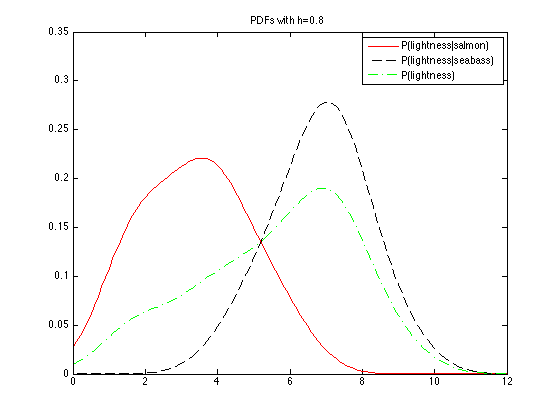
\includegraphics[scale=.57]{images/6_a.png}
  \caption{PDFs with h=0.8}
\end{figure}

\paragraph{b.} Plot of PDFs with h=0.2: \\

\begin{figure}[H]
  \centering
    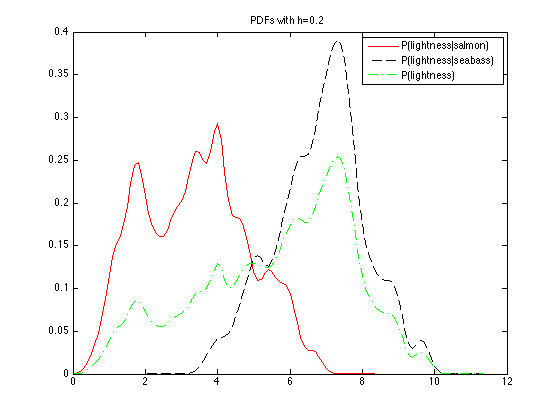
\includegraphics[scale=.57]{images/6_b.png}
  \caption{PDFs with h=0.2}
\end{figure}

\paragraph{c.} The glance into the above plots in (a) and (b) clearly reveals the effect of the difference in the window size parameter \textbf{h} of the Parzen-window method to learn the underlying distribution of the data. When in the case of $h=0.8$ the 3 PDFs namely $P(lightness|salmon)$, $P(lightness|seabass)$ and $P(lightness)$ is quite smooth comparing to when the $h=0.2$ which gives rather spiky distributions.


\newpage
\subsection*{Appendix:}
\lstinputlisting[language=Matlab, title=\lstname, basicstyle=\footnotesize]{assignment_4.m}
\lstinputlisting[language=Matlab, title=\lstname, basicstyle=\footnotesize]{problem_2.m}
\lstinputlisting[language=Matlab, title=\lstname, basicstyle=\footnotesize]{problem_3.m}
\lstinputlisting[language=Matlab, title=\lstname, basicstyle=\footnotesize]{problem_4.m}
\lstinputlisting[language=Matlab, title=\lstname, basicstyle=\footnotesize]{problem_5.m}
\lstinputlisting[language=Matlab, title=\lstname, basicstyle=\footnotesize]{problem_6.m}
\lstinputlisting[language=Matlab, title=\lstname, basicstyle=\footnotesize]{classify.m}
\lstinputlisting[language=Matlab, title=\lstname, basicstyle=\footnotesize]{g_mle.m}
\lstinputlisting[language=Matlab, title=\lstname, basicstyle=\footnotesize]{mle.m}
\lstinputlisting[language=Matlab, title=\lstname, basicstyle=\footnotesize]{parzen_window.m}

\lstinputlisting[language=Matlab, title=\lstname, basicstyle=\footnotesize]{pca_approximation.m}
\lstinputlisting[language=Matlab, title=\lstname, basicstyle=\footnotesize]{split.m}
\lstinputlisting[language=Matlab, title=\lstname, basicstyle=\footnotesize]{strcomp.m}






\end{document}